\subsection{Management persistenter Daten}

Die Speicherung der Daten erfolgt grundsätzlich in Form einer Datenbank für Kontakte mitsamt deren Chatverläufen und Nicknames. Des Weiteren gibt es \ac{CSQ} bzw. \ac{CRQ} und andere Dateien: Hash Chains der Kontakte, Directory (Info über Epochen) und Circuit Keys.
Das Kontaktbuch ist zweigeteilt, um Komplikationen zwischen den verschiedenen verwendeten Programmiersprachen bei gleichzeitigem Zugriff zu vermeiden. Deshalb gibt es eine KontaktID, welche zum Verbinden der Kontaktdaten dient.


\subsubsection{Verschlüsselung}
Die Verschlüsselung der persistenten Daten wird größtenteils vom Android Keystore System übernommen.
Dabei handelt es sich um einen von Android bereitgestellten Dienst, mit dessen Hilfe man kryptographische Schlüssel sicher abspeichern kann.
Zudem kann er auch benutzt werden, um Dateien verschlüsseln zu lassen.

Bei Dateien, welche vom Kotlin Teil verwaltet werden, wird die Verschlüsselung und das sichere Abspeichern der dafür benötigten Schlüssel komplett vom Keystore System übernommen.
Da die Verwendung des Keystore Systems bei C++ wesentlich schwieriger ist, als bei der Android nahestehenden Sprache Kotlin, wird hier anders verfahren.
Die Verschlüsselung der Dateien wird von eigenen Methoden der Core Bibliothek übernommen.
Der dafür notwendige Schlüssel wird vom Keystore System gespeichert und vom \ac{MS} bei C++ Methodenaufrufen als Parameter übergeben.

Sowohl das Keystore System, als auch die Core Bibliothek realisieren die Verschlüsselung durch AES.

\newpage
\subsubsection{Datenbank}
In der Datenbank ist das Kontaktbuch mit Kontakt IDs und dazugehörigen Nicknamen sowie Chatverläufen gespeichert.
Verschlüsselung erfolgt durch durch das Keystore System.
Zugriff erfolgt durch die \ac{GUI} und den \ac{MS}.

Das folgende ER-Modell beschreibt die Datenbank:

\begin{figure}[h]
  \centering
     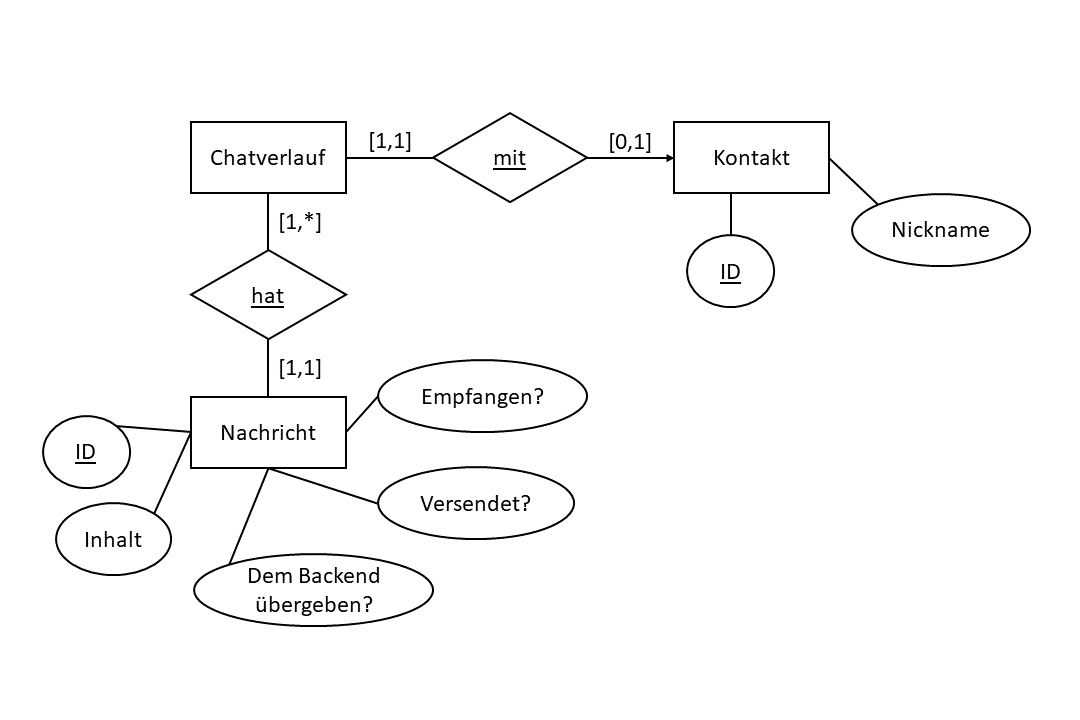
\includegraphics[width=0.9\textwidth]{diagramme/db.png}
  \caption{ER-Diagramm Datenbank}
  \label{fig:Bild8}
\end{figure}


\subsubsection{Kontakt Hash Chains}
\label{Kap2_3_2}
Im zweiten Teil des Kontaktbuchs sind Kontakt IDs mit zugehörigen gemeinsamen Schlüssel gespeichert.
Verschlüsselung erfolgt durch die Core Bibliothek.
Zugriff erfolgt durch das C++ Dateisystem.

\subsubsection{Directory}
Hier sind Informationen zu Epochen und Kommunikationsrunden gespeichert.
Da diese Daten öffentlich bekannt sind, ist diese Datei unverschlüsselt.
Zugriff erfolgt durch das C++ Dateisystem.

\subsubsection{Circuits}
In der Circuits Datei befinden sich die symmetrischen Schlüssel für die Mixe der gewählten Circuits für bestehende, sowie die kommenden Epochen.
Verschlüsselung erfolgt durch durch die Core Bibliothek.
Zugriff erfolgt durch das C++ Dateisystem.

\subsubsection{Cell Receive Queue}
\label{Kap2_3_6}
Dies ist eine Warteschlange, in der eingegangene, entschlüsselte Nachrichten, die noch entkomprimiert und ggf. defragmentiert werden müssen, zwischengespeichert werden.
Verschlüsselung erfolgt durch die Core Bibliothek.
Zugriff durch C++ Funktionen, die Verschlüsselung ausführen, sowie solche zur Fragmentierung und Komprimierung.

\subsubsection{Cell Send Queue}
Dies ist ein Warteschlange, in der komprimierte, ggf. fragmentierte Nachrichten, die versendet werden sollen, zwischengespeichert werden. 
Verschlüsselung erfolgt durch die Core Bibliothek.
Zugriff durch C++ Funktionen, die Verschlüsselung ausführen, sowie solche zur Fragmentierung und Komprimierung.
